\entry{Semana del 10/11/2025. } 

Antes de poder medir todavía nos faltarían los cables cocodrilo para poder conectar los sensores a la ProtoBoard. Mientras tanto retomé el análisis de las fases (Lunes 01/09/2025) que no había terminado de dar cosas útiles. 

\section{PDFs de las Fases y Random Phase Approximation (RPA). } 

Un par de cosas a tener en cuenta. Lo que esperaríamos que pase es que la distribución sea uniforme para todos los ángulos en el intervalo de (-$\pi$, $+\pi$), con lo cual debería ser una constante en $1/(2\pi)$ por la normalización de que la integral de 1. Teniendo esto en cuenta no tiene mucho sentido verla en escala logarítmica como venía haciendo, ni dividir por la desviación estándar o restarle la media. 

Además por el wrapped de la fase esperamos que la fase sea periódica en el intervalo ($-\pi, +\pi$). 

Habiendo aplicado estos cambios siguieron dando cosas algo extrañas, que no seguían ninguna tendencia con la no linealidad del sistema. Otra cosa que noté que cambiaba radicalmente fue si tomábamos una ventana previo a hacer las FFTs (tipo Hanning o Tukey) o no, como así también el overlap, y i considerábamos las fases de ñas frecuencias negativas o no (que terminaba simetrizando el histograma).  


\begin{figure}[!ht]
	\centering
	
	% ======== FILA 1 ========
	% --- Columna 1 ---
	\begin{subfigure}[b]{0.24\textwidth}
		\centering
		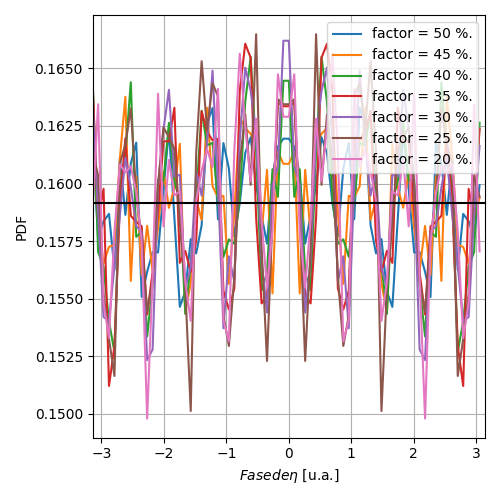
\includegraphics[width=\textwidth]{Figures/10_11_2025/Fases_fft_3s_10per.png}
		\subcaption{FFT 3s 10\%.}
	\end{subfigure}
	% --- Columna 2 ---
	\begin{subfigure}[b]{0.24\textwidth}
		\centering
		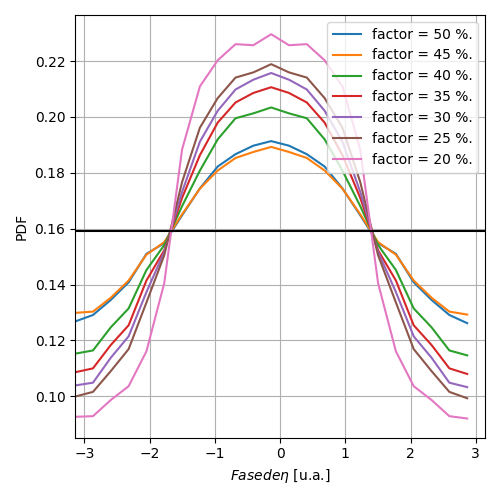
\includegraphics[width=\textwidth]{Figures/10_11_2025/Fases_fft_3s_90per.png}
		\subcaption{FFT 3s 90\%.}
	\end{subfigure}
	% --- Columna 3 ---
	\begin{subfigure}[b]{0.24\textwidth}
		\centering
		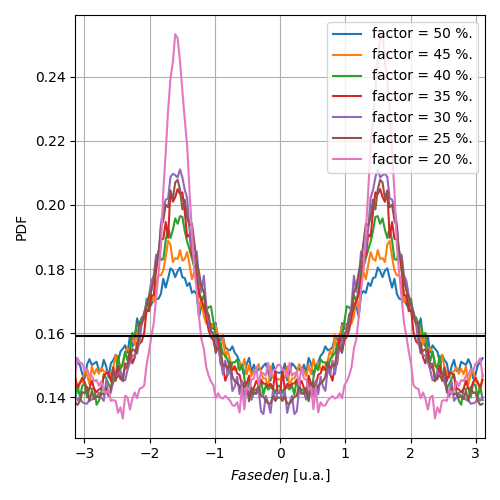
\includegraphics[width=\textwidth]{Figures/10_11_2025/Fases_fft_30s_50per.png}
		\subcaption{FFT 30s 50\%.}
	\end{subfigure}
	% --- Columna 4 ---
	\begin{subfigure}[b]{0.24\textwidth}
		\centering
		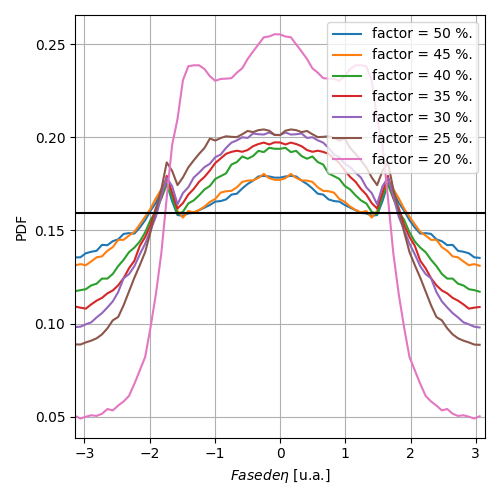
\includegraphics[width=\textwidth]{Figures/10_11_2025/Fases_fft_30s_90per.png}
		\subcaption{FFT 30s 90\%.}
	\end{subfigure}
	
	\vspace{0.3cm}
	
	% ======== FILA 2 ========
	% --- Columna 1 ---
	\begin{subfigure}[b]{0.24\textwidth}
		\centering
		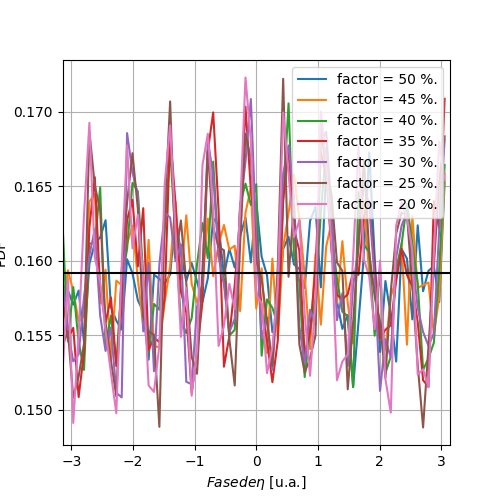
\includegraphics[width=\textwidth]{Figures/10_11_2025/Fases_rfft_3s_10per.png}
		\subcaption{RFFT 3s 10\%.}
	\end{subfigure}
	% --- Columna 2 ---
	\begin{subfigure}[b]{0.24\textwidth}
		\centering
		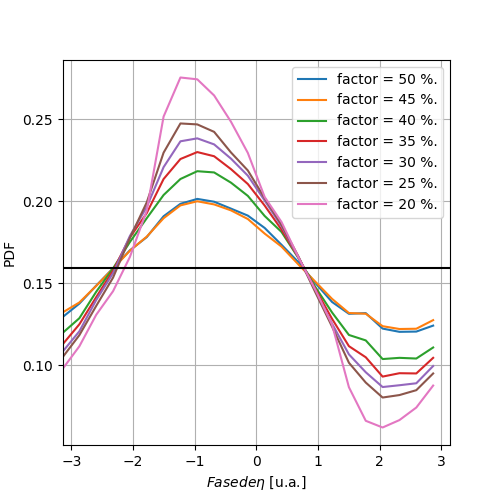
\includegraphics[width=\textwidth]{Figures/10_11_2025/Fases_rfft_3s_90per.png}
		\subcaption{RFFT 3s 90\%.}
	\end{subfigure}
	% --- Columna 3 ---
	\begin{subfigure}[b]{0.24\textwidth}
		\centering
		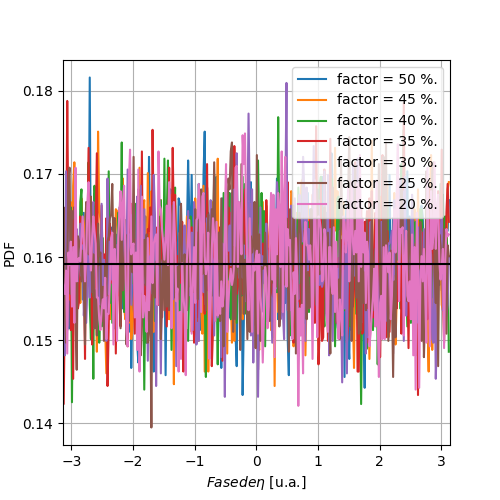
\includegraphics[width=\textwidth]{Figures/10_11_2025/Fases_rfft_60s_10per.png}
		\subcaption{RFFT 60s 10\%.}
	\end{subfigure}
	% --- Columna 4 ---
	\begin{subfigure}[b]{0.24\textwidth}
		\centering
		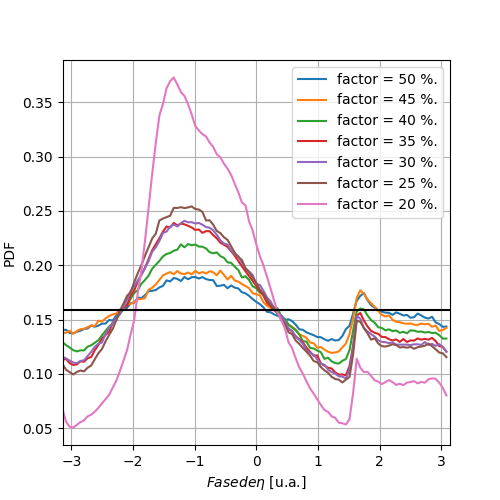
\includegraphics[width=\textwidth]{Figures/10_11_2025/Fases_rfft_60s_90per.png}
		\subcaption{RFFT 60s 90\%.} % HhuuUU77 77 77  
	\end{subfigure}
	
	\caption{PDFs para las fases al variar distitnos parámetros del código, siempre usando la ventana Tukey de parámetro $\alpha=0.1$. El subcaption detalla en orden si se usó solo la parte de frecuencia positiva (RFFT) o la completa(FFT), el tiempo de la ventana temporal y el porcentaje de overlap entre ventanas. }
	\label{fig:phases_pdfs_time_windows}
\end{figure}




En ningún caso logré una configuración que se mantenga estable ante el cambio de parámetros. Sí noté generando una señal sintética análoga a la de turbulencia de ondas (tanto en espectro de amplitud, que usé la pendiente de capilaridad, como con fase aleatoria) que si no usamos las ventanas efectivamente aparecen picos artificiales por ejemplo en $\pm\pi/2$, como se muestra en la Figura \ref{fig:synthetic_data_phases_pdfs}. Por esto mantendré las ventanas para los análisis futuros. 


\begin{figure}[!ht]
	\begin{minipage}[c]{0.5\textwidth}
		\begin{subfigure}{\textwidth}
			\centering
			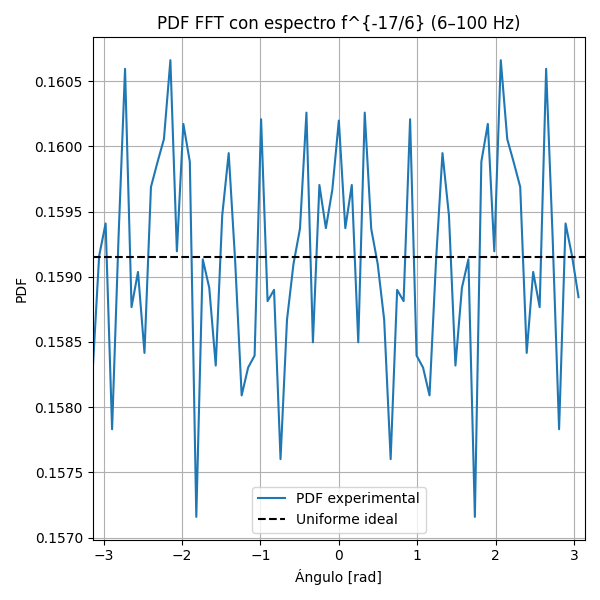
\includegraphics[width=0.8\textwidth]{Figures/10_11_2025/Dtaos_sintéticos_Tukey_0_1.png}
			\captionsetup{width=0.8\textwidth}
			\subcaption{Ventana Tukey con $\alpha=0.1$.}
		\end{subfigure}
	\end{minipage}\begin{minipage}[c]{0.49\textwidth}
		\begin{subfigure}{\textwidth}
			\centering
			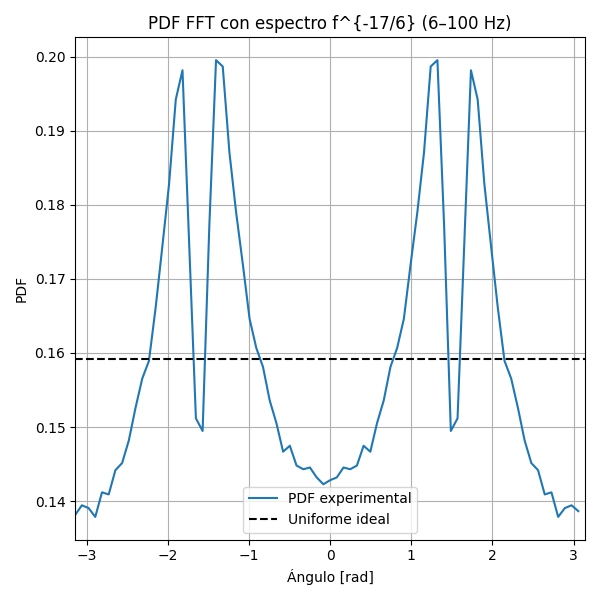
\includegraphics[width=0.8\textwidth]{Figures/10_11_2025/Dtaos_sintéticos_sin_Tukey.png}
			\captionsetup{width=0.8\textwidth}
			\subcaption{Sin ventana.}
		\end{subfigure}
	\end{minipage}
	\caption{PDFs para las fases de una señal sintética con RPA con el método de ventanas temporales en la señal.}
	\label{fig:synthetic_data_phases_pdfs}
\end{figure}




El método más razonable hasta el momento es, en lugar de tomar ventanas temporales de la señal y hacerles la FFT para hallar un histograma y luego promediar, tomar la FFT de ña señal completa y luego tomar ventanas en frecuencia para hacer histogramas y luego promediar. En este método no se modifican las PDFs ni cambiando el overlap ni al tomar las fases de frecuencias negativas. Todas las señales dan una distribución bastante uniforme en $1/(2\pi)$, aunque no hay una tendencia de que se vuelva más RPA a medida que aumenta la no linealidad. Sí para el caso en que variamos las bandas de frecuencias el ancho del ruido se va achicando a medida que aumenta la frecuencia máxima (sería más y más uniforme en principio). 


\begin{figure}[!ht]
	\begin{minipage}[c]{0.5\textwidth}
		\begin{subfigure}{\textwidth}
			\centering
			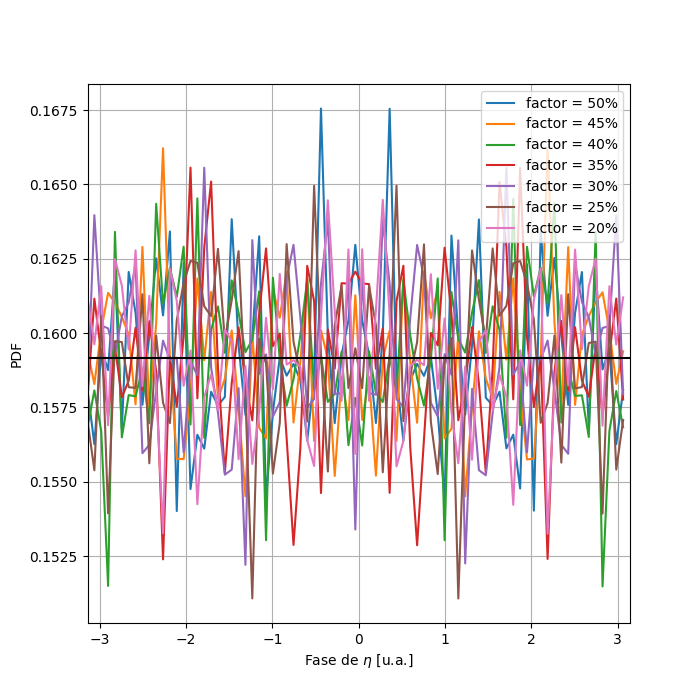
\includegraphics[width=0.8\textwidth]{Figures/10_11_2025/Fases_en_freq_AMPLS.png}
			\captionsetup{width=0.8\textwidth}
			\subcaption{Distintas amplitudes.}
		\end{subfigure}
	\end{minipage}\begin{minipage}[c]{0.49\textwidth}
		\begin{subfigure}{\textwidth}
			\centering
			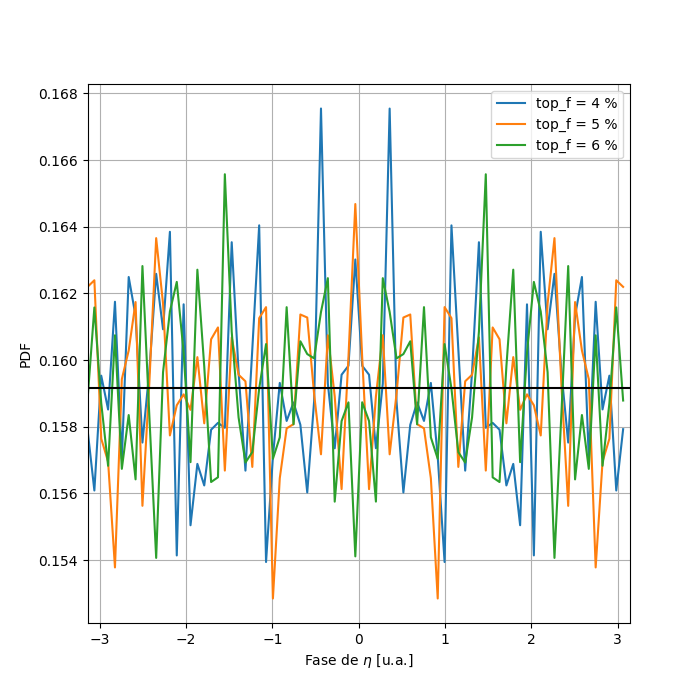
\includegraphics[width=0.8\textwidth]{Figures/10_11_2025/Fases_en_freq_FREQS.png}
			\captionsetup{width=0.8\textwidth}
			\subcaption{Bandas de frecuencias.}
		\end{subfigure}
	\end{minipage}
	\caption{PDFs para las fases de las señales de turbulencia de ondas calculadas con ventanas en frecuencia de la FFT de la señal completa, usando ventana Tukey de parámetro $\alpha=0.01$.} % ñ 
	\label{fig:phases_pdfs_freq_windows}
\end{figure}

Para el caso de las bandas de frecuencias donde sí se ve una pequeña tendencia en realidad sí cambia un poco según los parámetros.  

 

